\documentclass[10pt,aspectratio=169, colorlinks=true, linkcolor=circlBlue]{beamer}

% tlp allowed values: clear, green, amber, amber+strict, red
\usetheme[numbering=fraction, progressbar=frametitle, tlp=clear]{circl}

% for code highlighting
\usepackage{minted}
% to draw pingus
\usepackage{tikzpingus}
% to draw boxes to catch attention
\usepackage{awesomebox}
% For hyperlinks in the document and PDF metadata
\usepackage{hyperref}
% useful only if we want to customize minted background
\usepackage{tcolorbox}

\usepackage{multicol}
%
% compile with -shell-escape in order to use minted
% $ pdflatex  -interaction=nonstopmode -shell-escape presentation.tex
%


\hypersetup{
    pdftitle={AIL Project - Practical and Efficient Data-Mining of Chats, Suspicious Websites, Forums and Tor Hidden-Services},    % Title
    pdfauthor={Aurelien Thirion, Alexandre Dulaunoy},               % Author
    pdfsubject={Practical and Efficient Data-Mining of Chats, Suspicious Websites, Forums and Tor Hidden-Services}, % Subject
    pdfkeywords={ail-project, AIL}, % Keywords
    colorlinks=false,                       % Color links instead of boxes
    linkcolor=blue,                        % Color of internal links
    citecolor=blue,                        % Color of citations
    urlcolor=blue                          % Color of external links
}

% set the logo to put in the title page
\titlegraphic{\noindent
\includegraphics[width=0.25\textwidth]{images/logo-circl.pdf}\hfill
\includegraphics[height=0.12\textwidth]{images/ail-project.png}}
\title{AIL Project - Practical and Efficient Data-Mining of Chats, Suspicious Websites, Forums and Tor Hidden-Services}
\subtitle{CIRCL - Virtual Summer School 2025}
\date{July 17, 2025}
\author{Alexandre Dulaunoy - alexandre.dulaunoy@circl.lu\\Aurelien Thirion - aurelien.thirion@circl.lu}
\institute{CIRCL \normalurl{https://www.circl.lu}}
% if set inserts a title link into the title page
\titlelink{\faHome\space \normalurl{https://ail-project.org/}}

\begin{document}

% include custom commands

% Place here your custom commands, it will be included in presentation.tex

\newcommand{\normalurl}[1]{\href{#1}{#1}}

\newcommand{\footnoteurl}[1]{\footnote{\scriptsize\url{#1}}}

\newcommand{\rocketbox}[1]{%
	\awesomebox[circlRed]{1pt}{\faRocket}{circlBlue}{#1}%
}


% Title page
\begin{frame}
	\titlepage%
\end{frame}


% --------- Summary ---------
%\setcounter{tocdepth}{2}
%\begin{frame}
%    \frametitle{Content at glance}
%    \tableofcontents
%\end{frame}
%\setcounter{tocdepth}{4}
% ----------------------------


\begin{frame}
    \frametitle{Background}
    \begin{itemize}
        \item Over the past years, CIRCL has developed the AIL project\footnote{\url{https://www.ail-project.org/}} to fulfill our needs at CIRCL in intelligence gathering and analysis.
        \item AIL features an extensible Python-based framework for the \textbf{analysis of unstructured information}, collected either through an advanced crawler manager or from various feeders, including social networks and custom feeders.
        \item The AIL Project is an \textbf{open-source} framework\footnote{\url{https://github.com/ail-project}} comprising various modules designed for the \textbf{collection, crawling, digging, and analysis of unstructured data}.
        \item 
            \begin{figure}
                \centering
                
\includegraphics[scale=0.1]{images/ail-project.png}
            \end{figure}
    \end{itemize}
\end{frame}

% collection issue

\begin{frame}
    \frametitle{High Level Overview}
    \begin{center}
        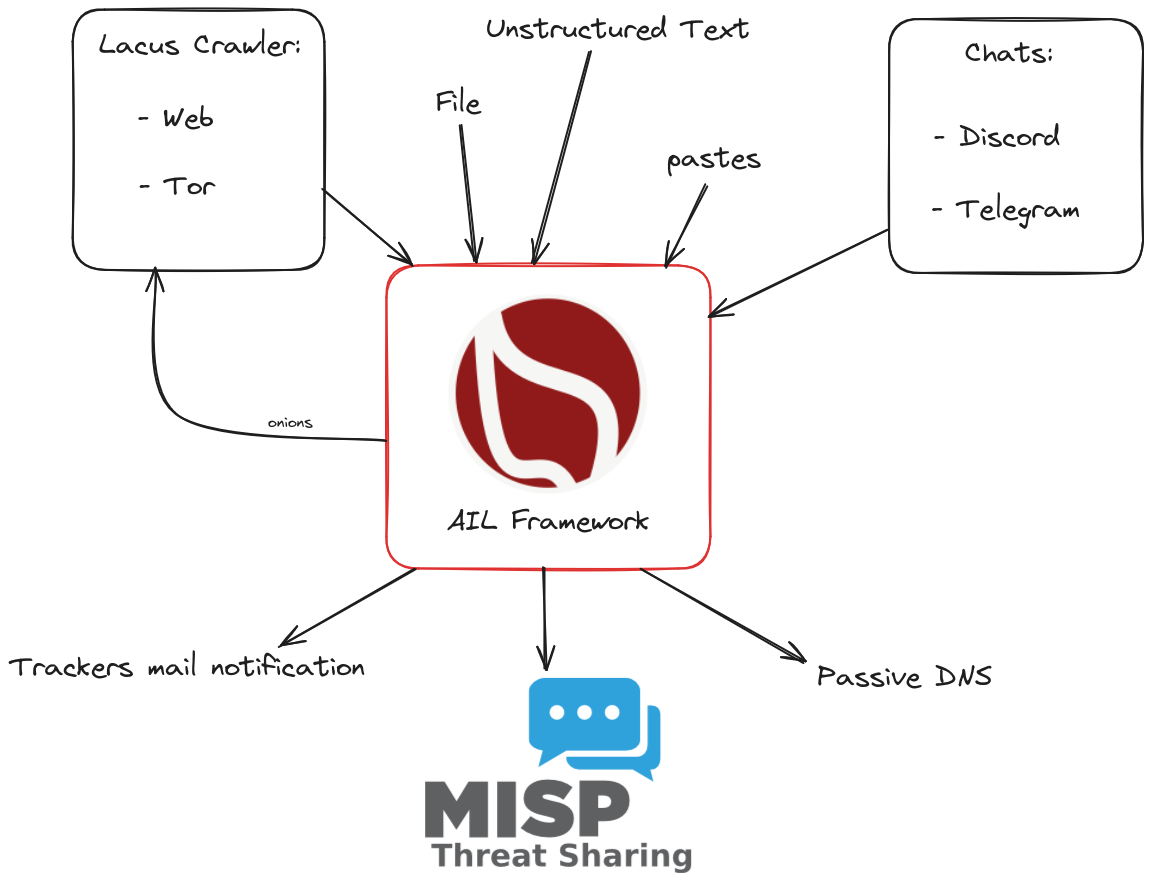
\includegraphics[scale=0.24]{images/ail-overview.png}
    \end{center}
\end{frame}


\begin{frame}
    \frametitle{Analysis of unstructured information}
    \begin{center}
        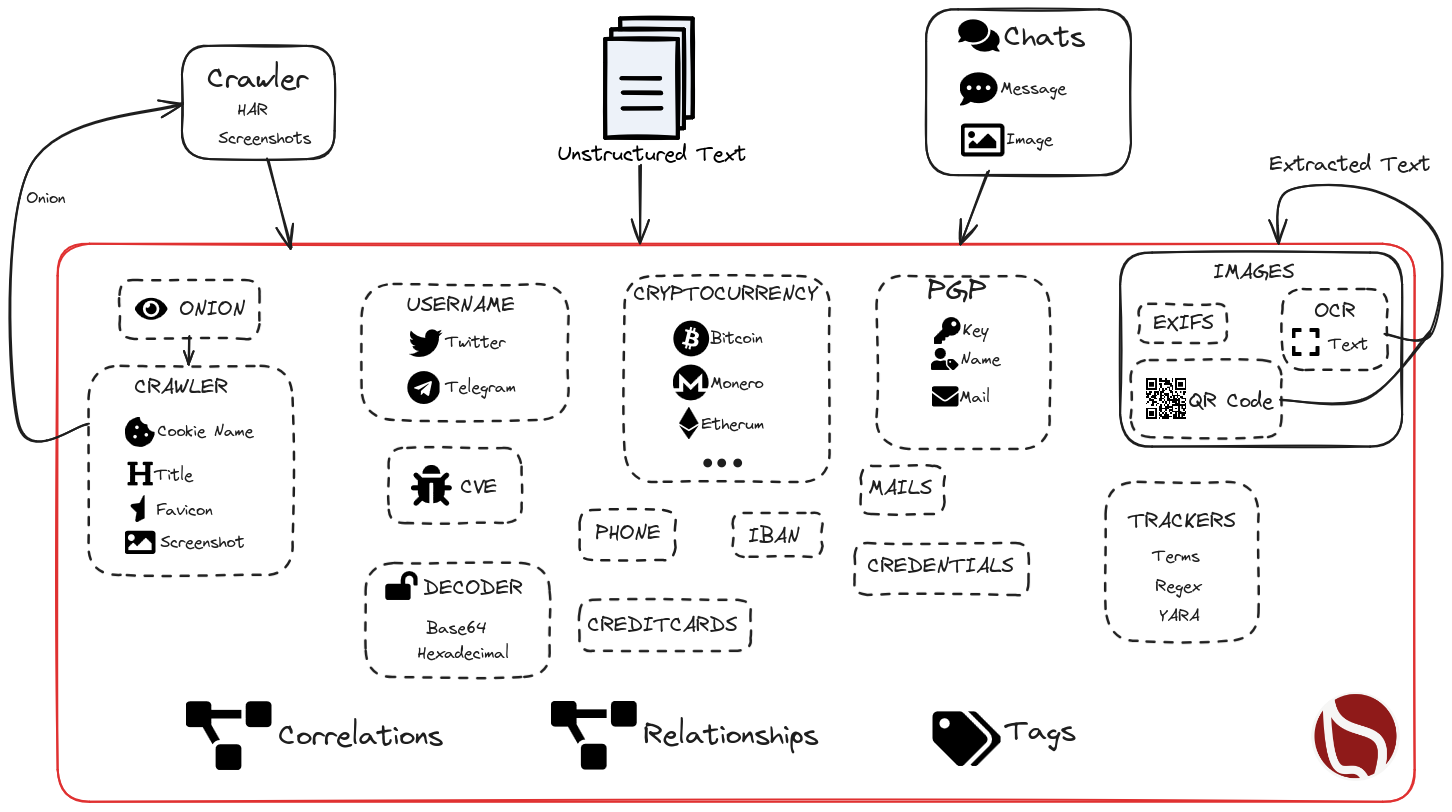
\includegraphics[scale=0.225]{images/ail-internal.png}
    \end{center}
\end{frame}

\begin{frame}
    \frametitle{{\it Collection} - automate crawling}

\begin{itemize}
    \item Crawling can be a challenging task, for example, gathering all the blog posts from ransomware groups\footnote{\url{https://www.ransomlook.io/}}, which can be demanding for an analyst.
    \item AIL offers a crawling feature that can {\bf initiate regular crawls using a standard spawned browser}.
\end{itemize}
    \begin{center}
        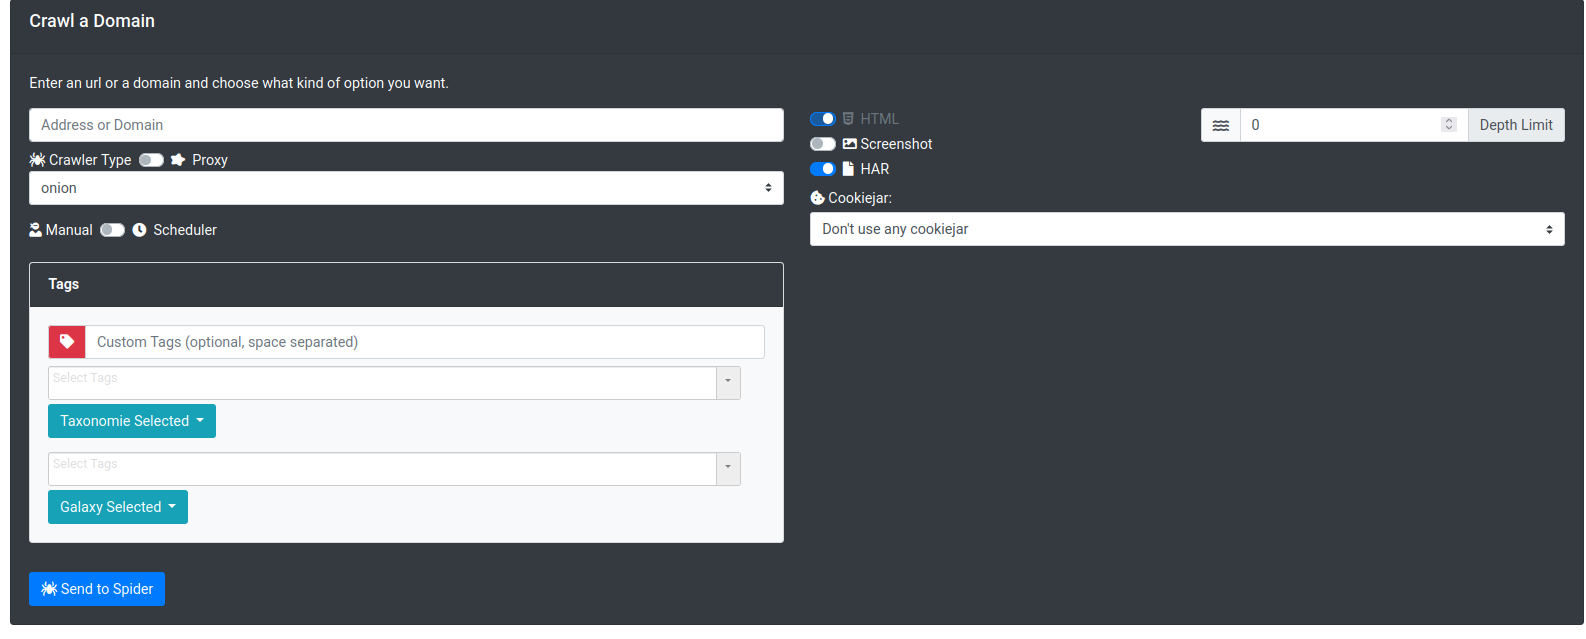
\includegraphics[scale=0.17]{images/ail-crawling.png}
    \end{center}
\end{frame}

\begin{frame}
    \frametitle{{\it Collection} - Lacus Crawler\footnote{\url{https://github.com/ail-project/lacus}}}
        	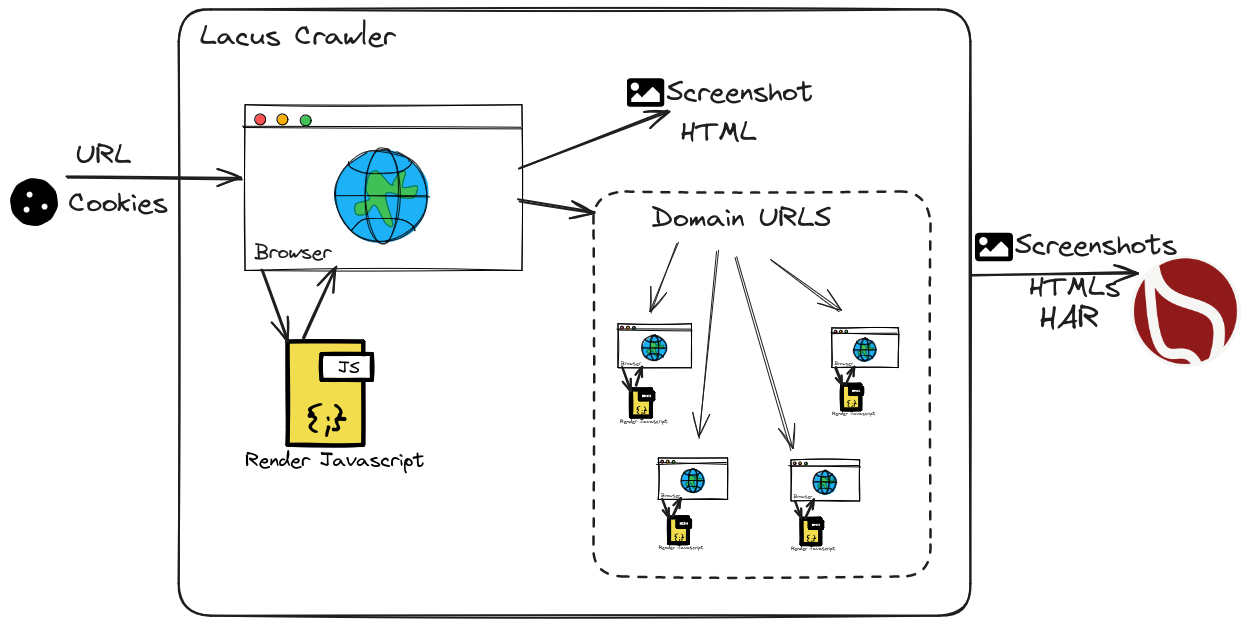
\includegraphics[scale=0.27]{images/ail-lacus.png}
\end{frame}


\begin{frame}
    \frametitle{Crawler: Cookiejar}
    Use your cookies to login and bypass captcha
    \centerline{
        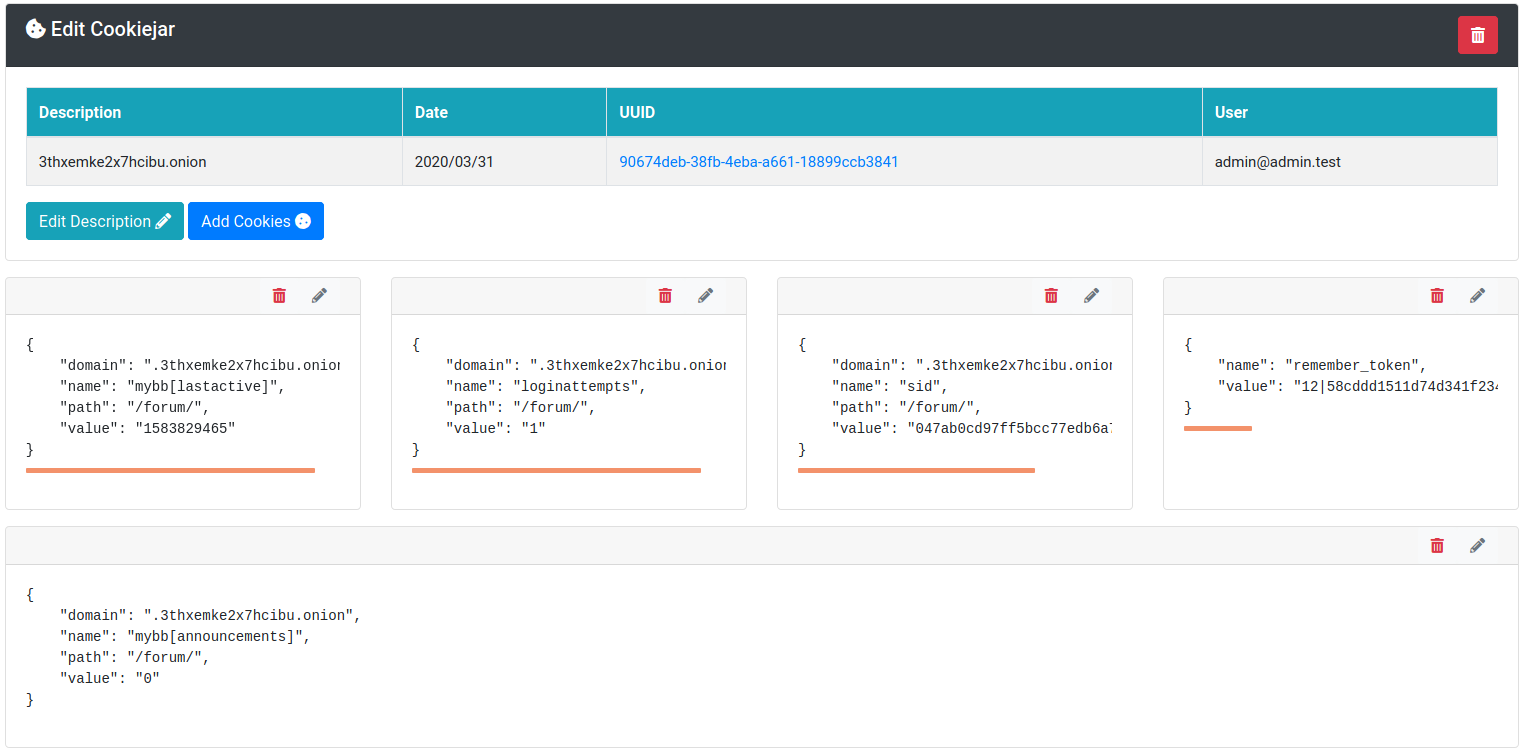
\includegraphics[scale=0.23]{screenshot/crawler-cookiejar-edit.png}
    }
\end{frame}

\begin{frame}
    \frametitle{Crawler: Cookiejar}
    \centerline{
        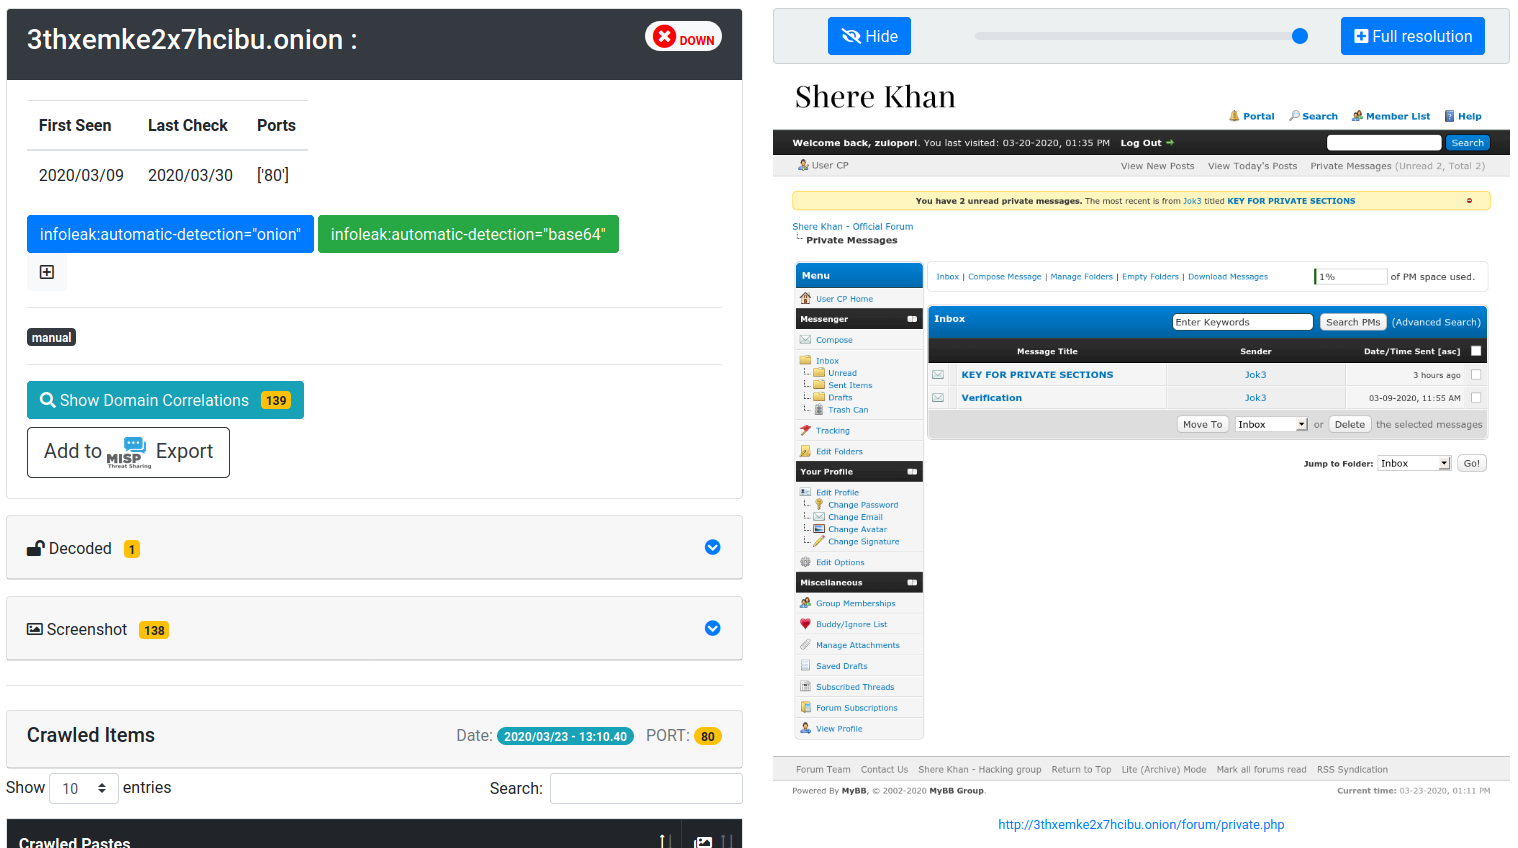
\includegraphics[scale=0.23]{screenshot/crawler-cookiejar-domain-crawled.png}
    }
\end{frame}

\begin{frame}
    \frametitle{Onion Lookup - onion.ail-project.org}

    \begin{itemize}
        \item \url{https://onion.ail-project.org} is a public search engine powered by AIL.
        \item Check if a Tor hidden service exists and retrieve its associated metadata.
        \item Can be used to filter onion domains related to CSAM and other violent content.
    \end{itemize}

    \begin{center}
        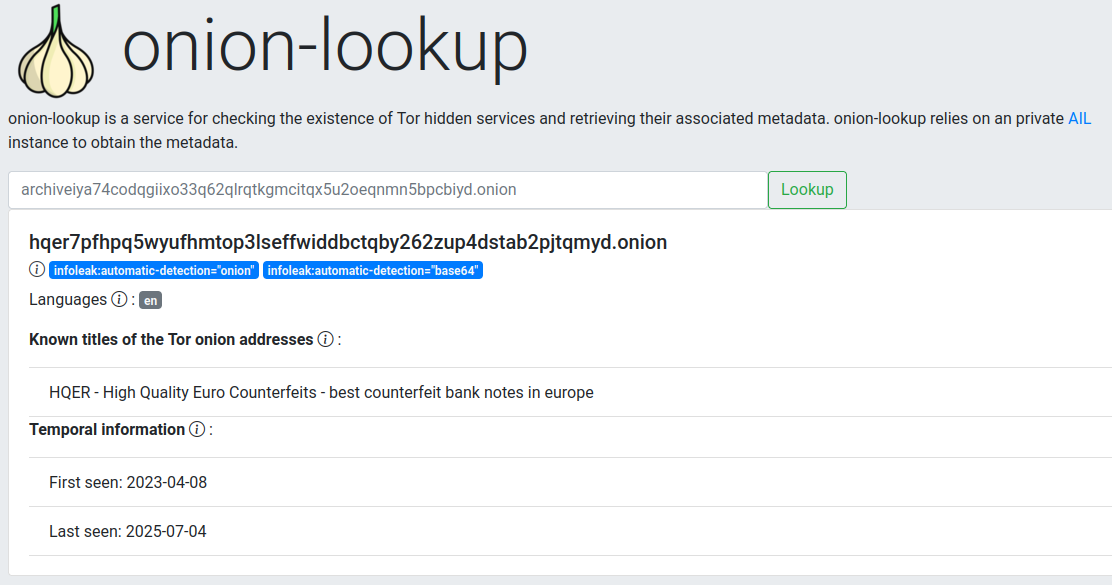
\includegraphics[scale=0.26]{images/onion-lookup.png}
    \end{center}
\end{frame}

\begin{frame}
    \frametitle{Crawler - Pre-Filtering }
    \begin{center}
        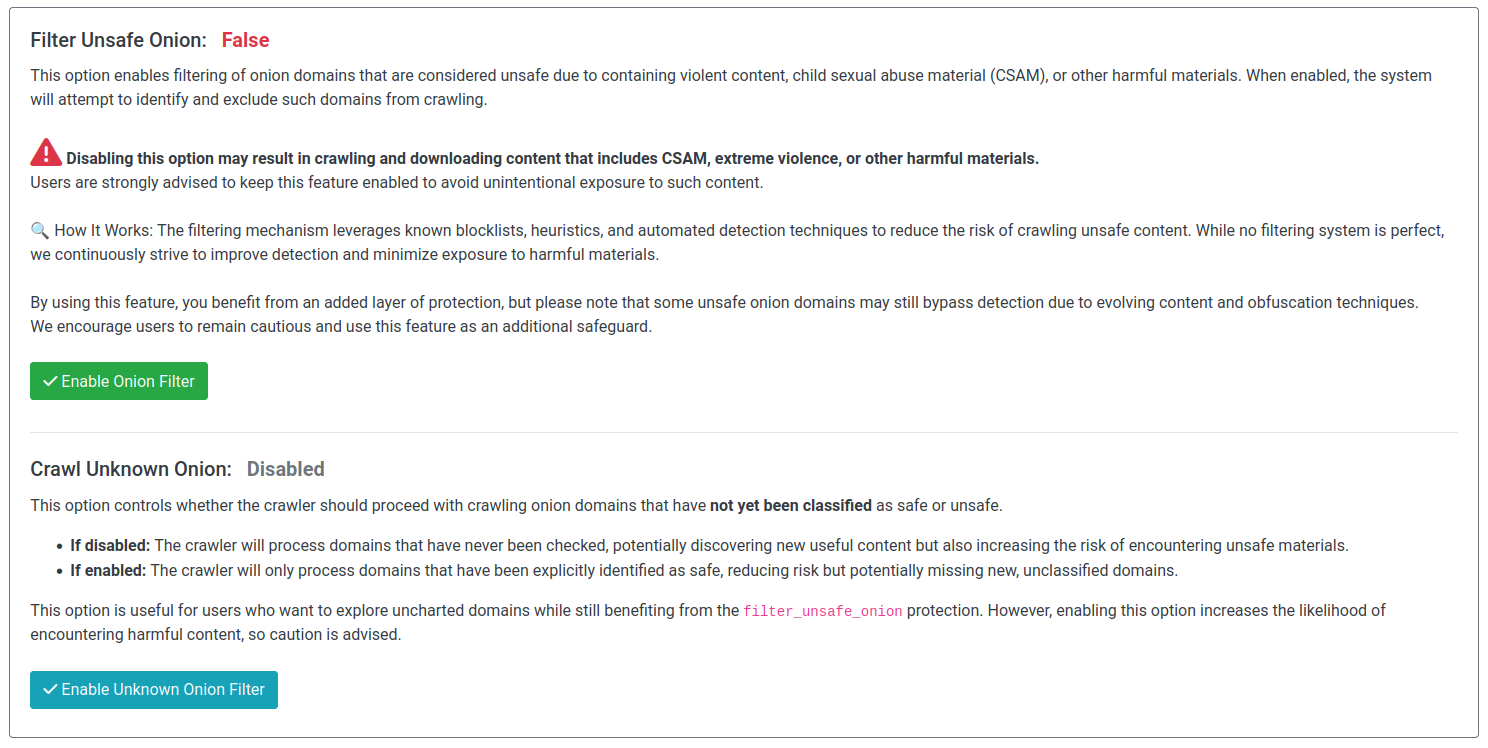
\includegraphics[scale=0.27]{images/ail-crawler-filter.png}
    \end{center}
\end{frame}

\begin{frame}
    \frametitle{\textit{Collection} - Automate Collection}
    \begin{itemize}
        \item Collecting data from various chat sources can be a \textbf{tedious task for analysts}.
        \item AIL offers a set of feeders (e.g., Telegram, Discord) that can be used to subscribe to chat channels.
        \item All the \textbf{collected messages are then processed and analyzed} within AIL's \textit{processing} and \textit{analysis} stages.
    \end{itemize}
    \begin{center}
        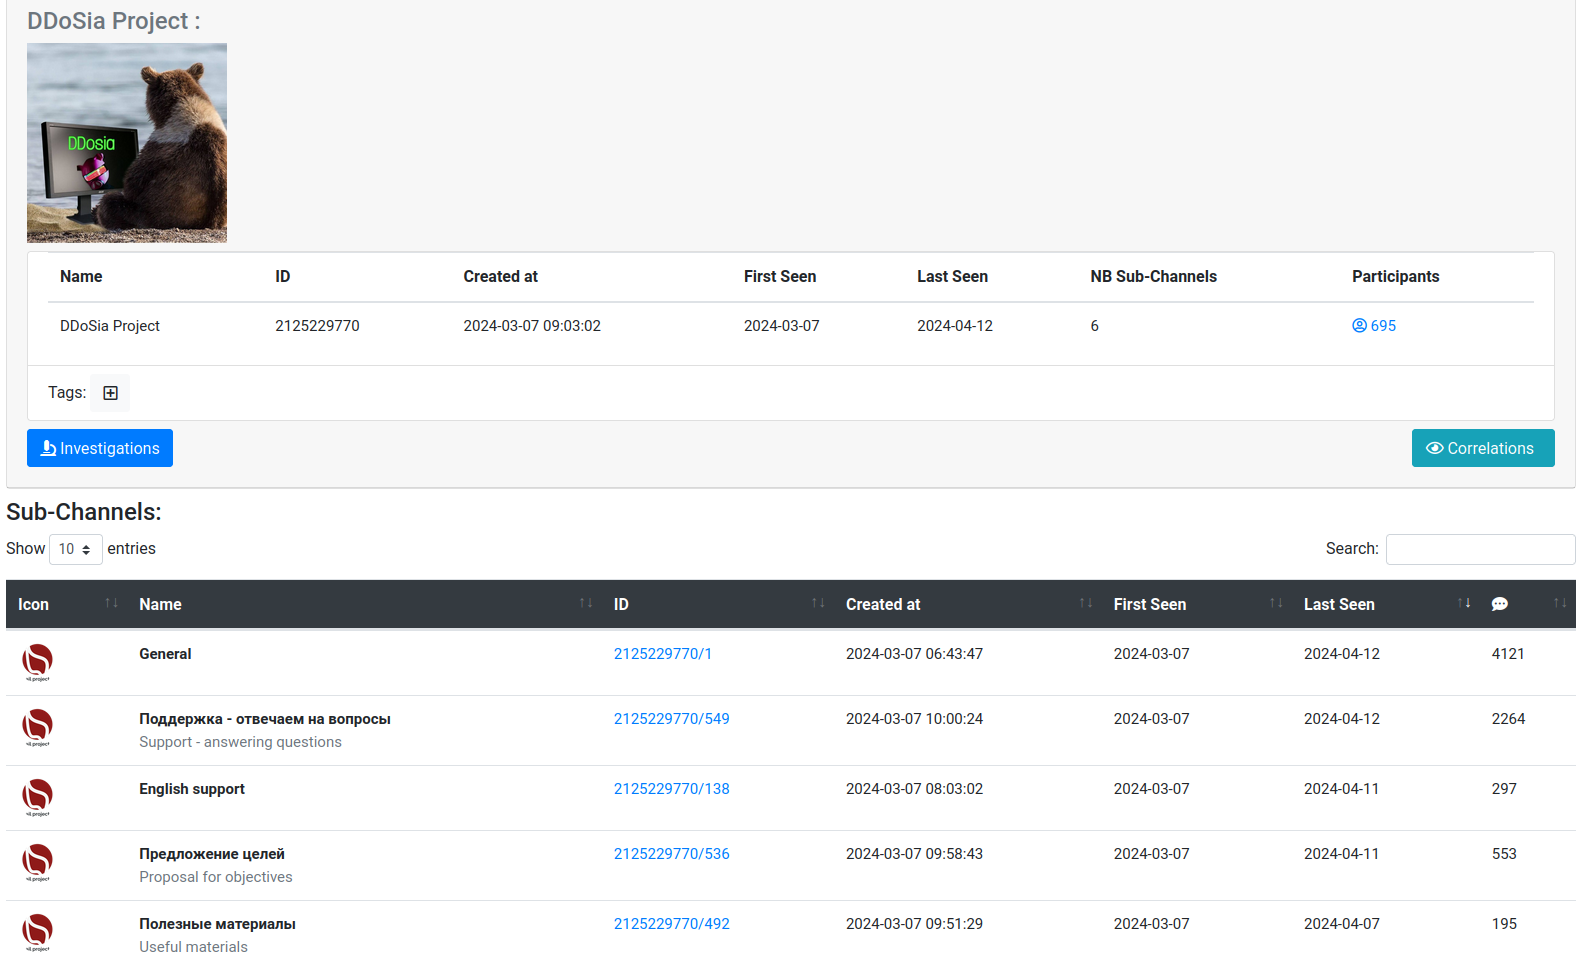
\includegraphics[scale=0.18]{screenshot/chat-forum.png}
    \end{center}
\end{frame}

% TODO Processing ISSUES
%\begin{frame}
%    \frametitle{{\it Processing - Chats TODO GRAPH}}
%	\begin{itemize}
%		\item Processing automatically collected information can be a challenging task.
%		\item Chats image + description 
%		\item user image + description 
%		\item message + meta
%	\end{itemize}
%\end{frame}

\begin{frame}[fragile]{OCR: Optical Character Recognition}
    \begin{columns}[T,onlytextwidth]
        \column{0.45\textwidth}
            \centering
            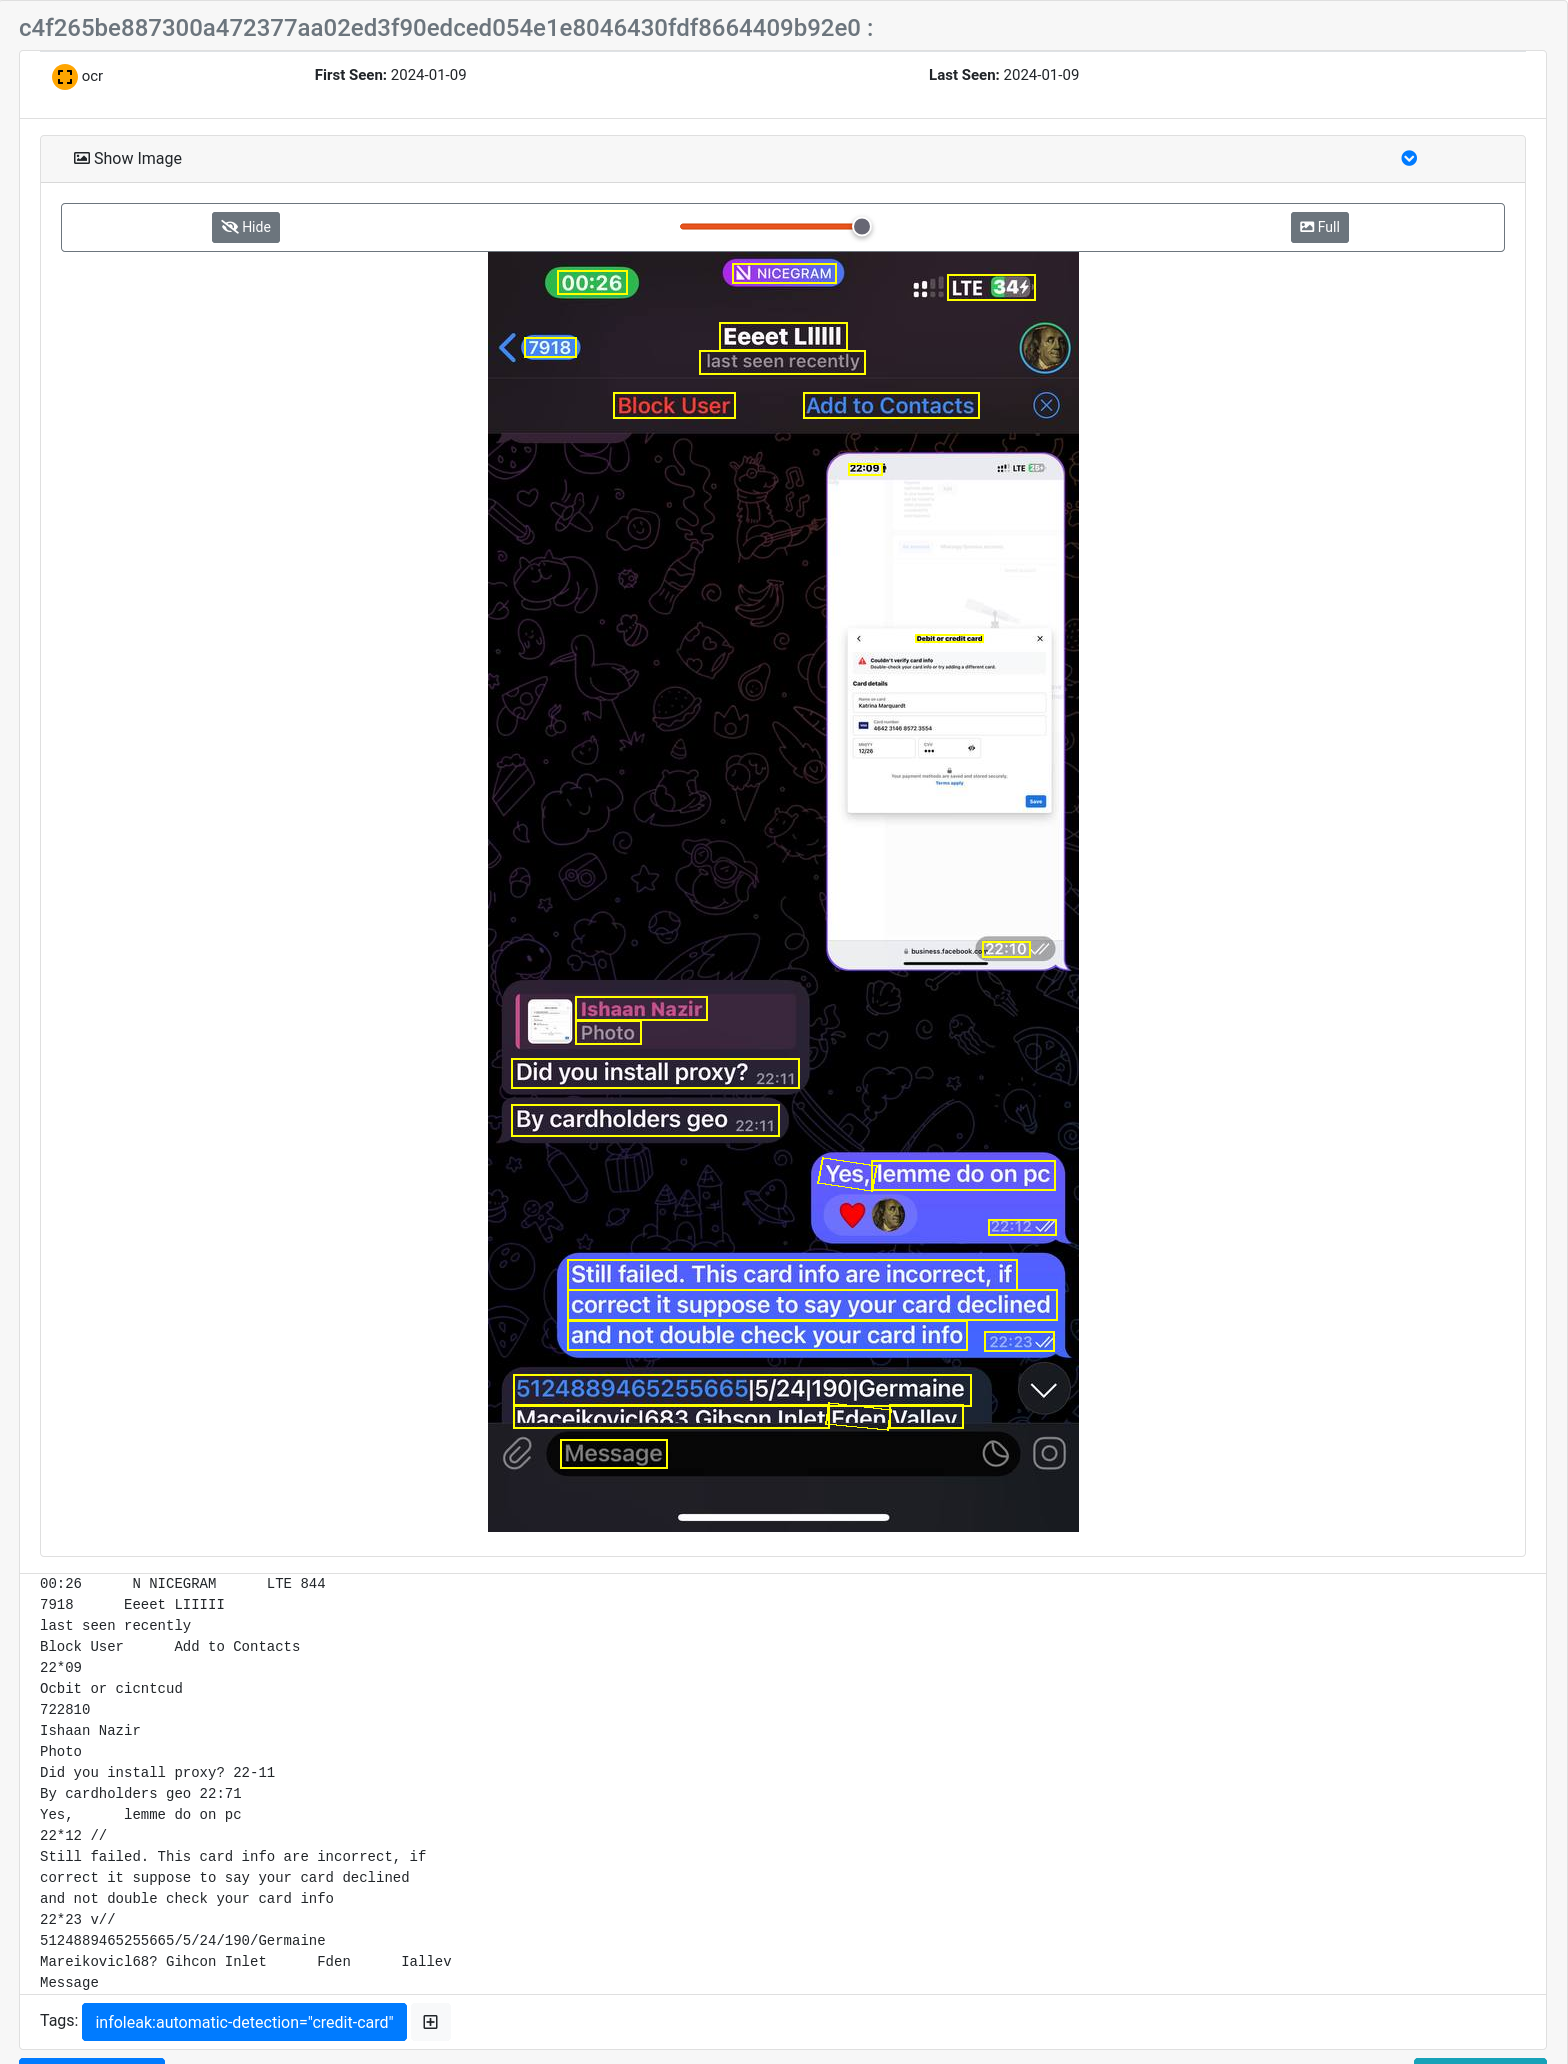
\includegraphics[width=\linewidth]{screenshot/ocr-1.png}
        \column{0.55\textwidth}
            \begin{itemize}
                \item Threat actors are often verbose and frequently {\bf share extensive details in private channels}.
                \item Many messages contain screenshots and images.
                \item Text detection and extraction are performed across 80+ languages using a CRNN (Convolutional Recurrent Neural Network).
                \item {\bf Enables keyword-based matching and detection}.
            \end{itemize}
    \end{columns}
\end{frame}

\begin{frame}
    \frametitle{QR Code Extractor}
    \begin{center}
        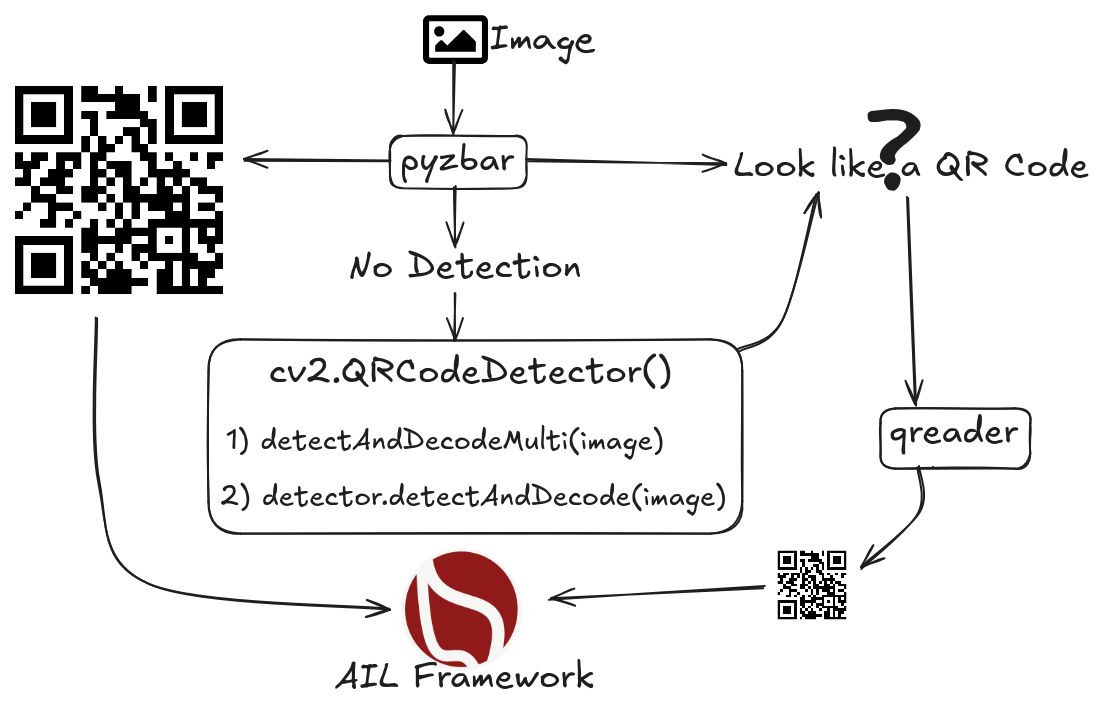
\includegraphics[scale=0.27]{images/qr_decoder.png}
    \end{center}
\end{frame}

\begin{frame}[fragile]{QR Codes}
    \begin{center}
        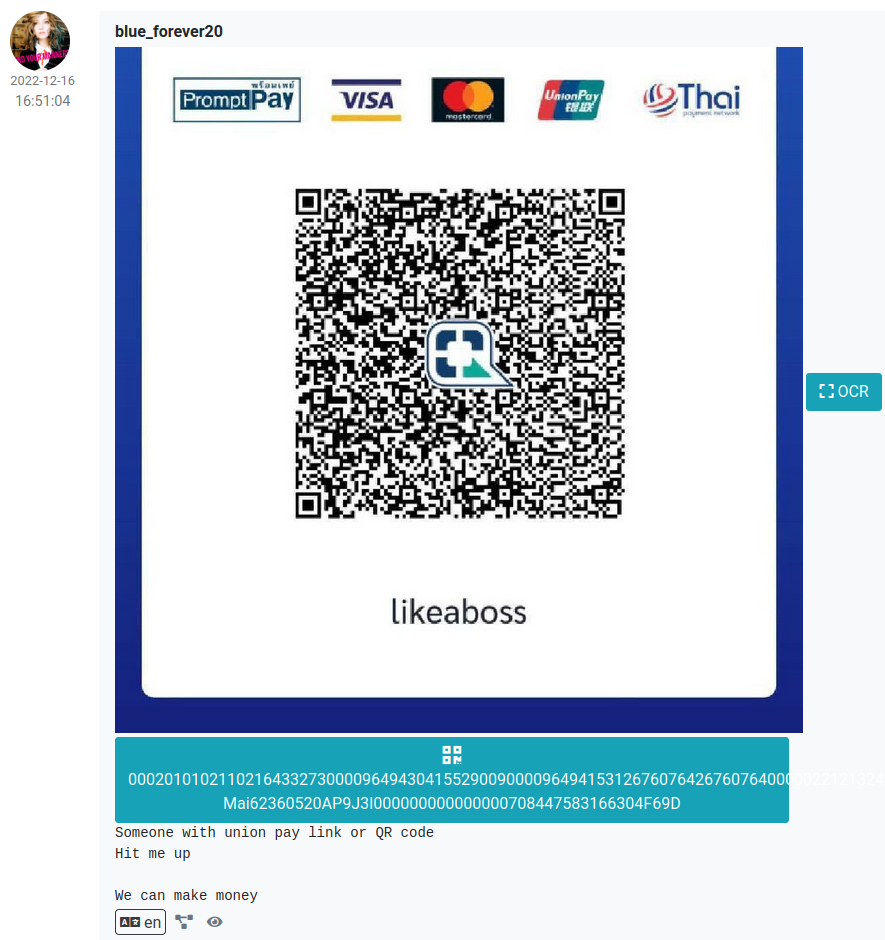
\includegraphics[scale=0.235]{screenshot/qr-pay.png}
    \end{center}
\end{frame}

\begin{frame}[fragile]{Bar Codes}
    \begin{center}
        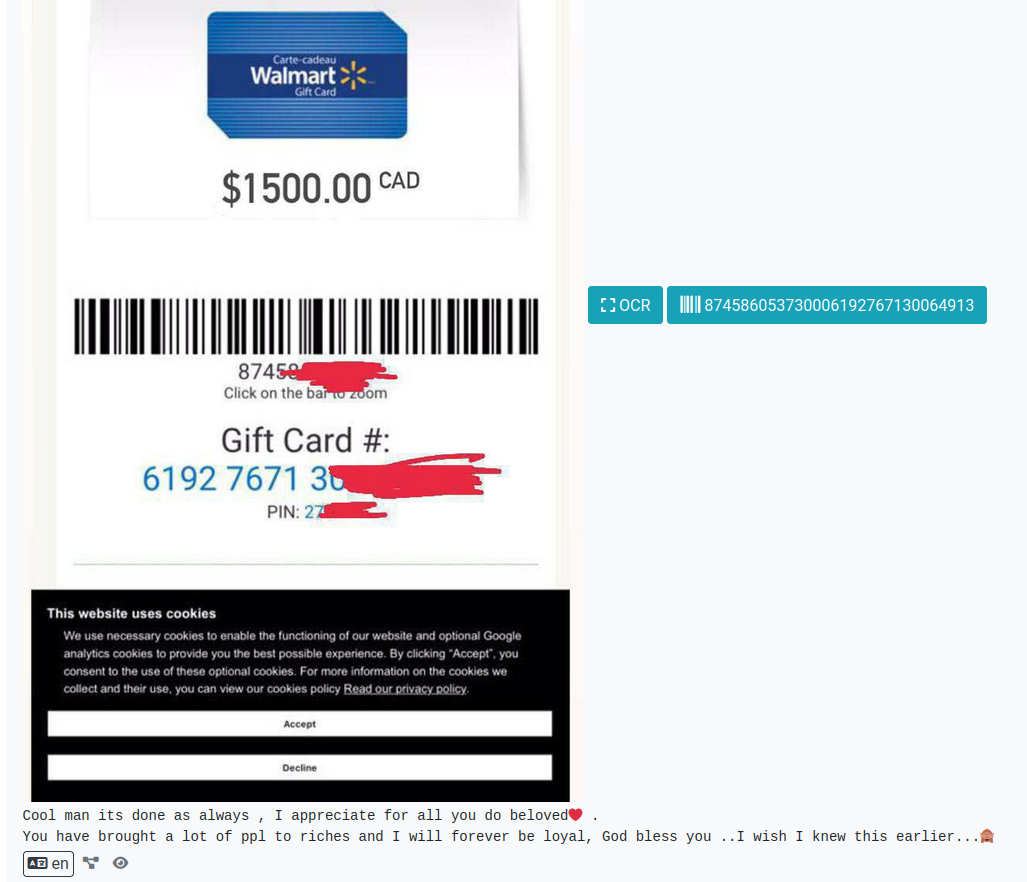
\includegraphics[scale=0.22]{screenshot/barcode.png}
    \end{center}
\end{frame}

\begin{frame}[fragile]{Images Descriptions}
    \begin{itemize}
        \item Uses \textbf{Ollama} and \textbf{Qwen2.5-VL} to automatically generate descriptions for screenshots and other images.
    \end{itemize}
    \begin{center}
        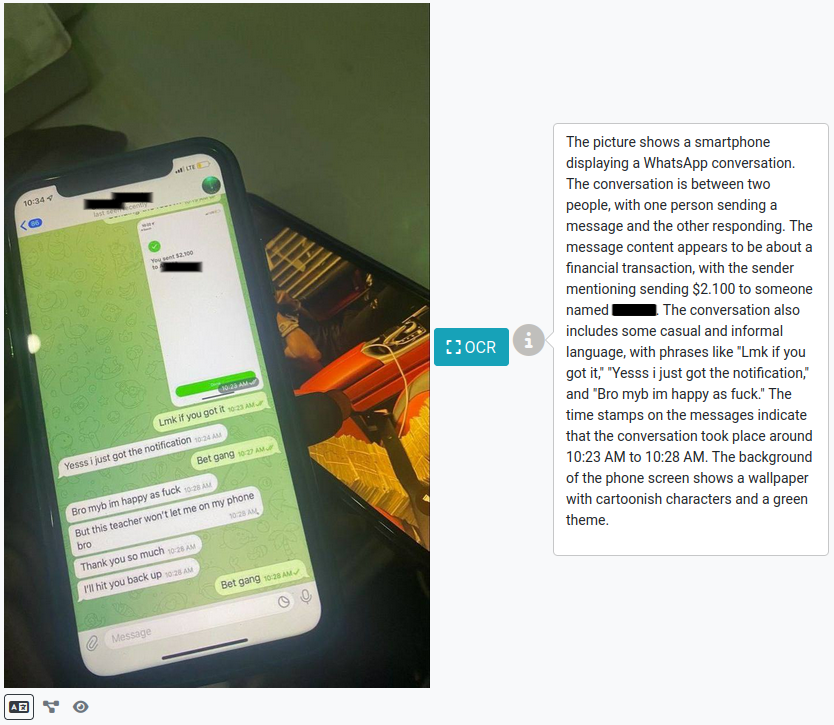
\includegraphics[scale=0.25]{images/image-description-phone.png}
    \end{center}
\end{frame}

\begin{frame}[fragile]{Images Descriptions}
    \begin{itemize}
    	\item Helps users quickly understand image content without viewing the image directly.
        \item Generated descriptions provide an extra layer of insight during analysis.
    \end{itemize}
    \begin{center}
        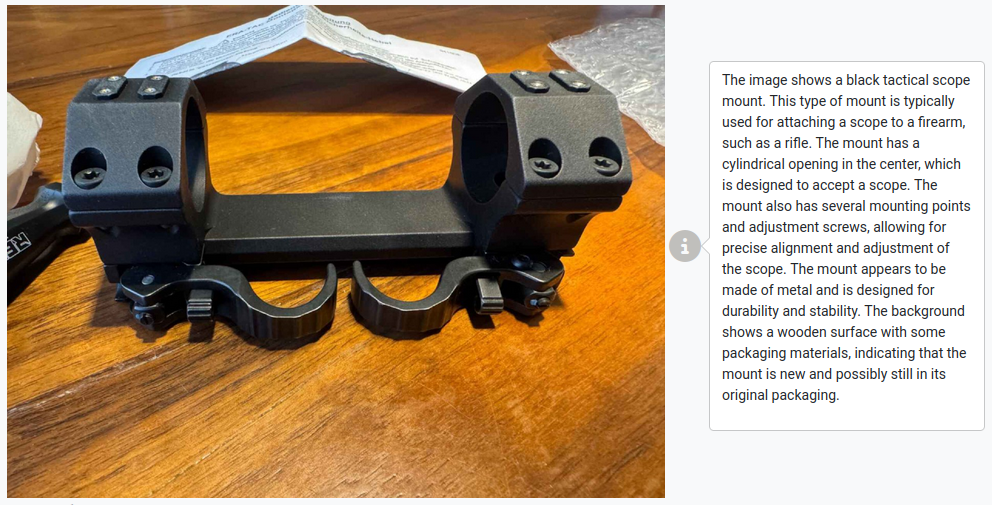
\includegraphics[scale=0.32]{images/image-description-mount.png}
    \end{center}
\end{frame}

\begin{frame}
    \frametitle{AIL Framework: Features}
    \begin{itemize}
        \item Extracting \textbf{credit card numbers, credentials, phone numbers, \dots}
        \item Extracting and validating potential \textbf{hostnames}
        \item Submission to threat sharing and incident response platforms (\textbf{MISP} and \textbf{FlowIntel}\footnote{\url{https://github.com/flowintel/flowintel}})
        \item \textbf{Tagging}\footnote{Relying on MISP taxonomies and galaxy} for classification and searches
        \item Terms, sets, regex, and YARA \textbf{tracking, occurrences, and history}
        \item Archives, files, and raw \textbf{submission} from the UI
        \item Correlation engine based on PGP ID, cryptocurrencies, decoded (Base64, \dots), usernames, cookie names, and many selectors to find relationships
        \item And many more
    \end{itemize}
\end{frame}


\begin{frame}
	\frametitle{Live Trackers \& Retro Hunt}
    \begin{itemize}
        \item Search and monitor specific keywords/patterns
        \begin{itemize}
            \item Automatic tagging
            \item Email/webhook notifications
        \end{itemize}
        \item Track Word
        \begin{itemize}
            \item ddos
        \end{itemize}
        \item Track Set
        \begin{itemize}
            \item booter, ddos, stresser; 2
        \end{itemize}
        \item Track Regex
        \begin{itemize}
            \item circl\textbackslash lu
        \end{itemize}
        \item {\bf YARA rules}
        \begin{itemize}
            \item \url{https://github.com/ail-project/ail-yara-rules}
        \end{itemize}
    \end{itemize}
\end{frame}

\section{Live Demo}

\begin{frame}
    \frametitle{Dashboard}
    \begin{figure}
        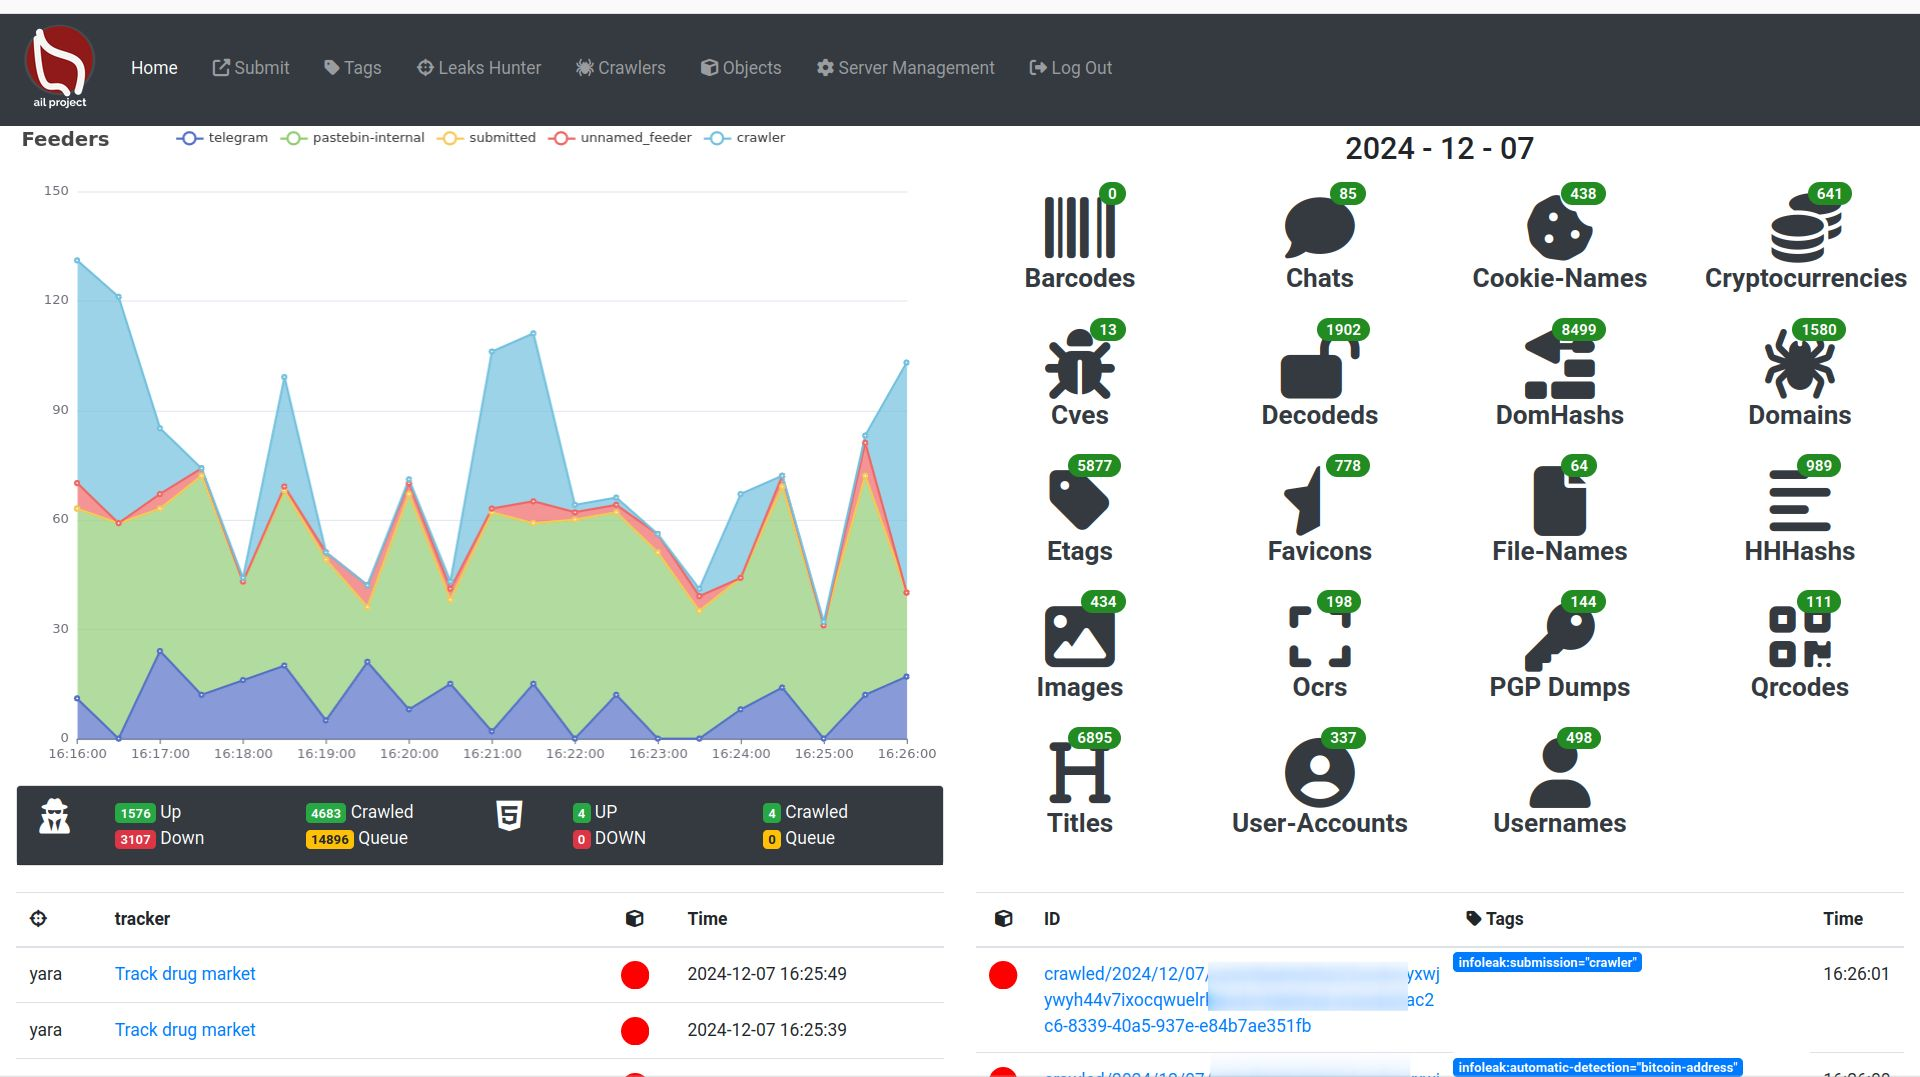
\includegraphics[scale=0.16, angle=0]{screenshot/dashboard.jpeg}
    \end{figure}
\end{frame}

\begin{frame}
    \frametitle{Search}
    \begin{figure}
        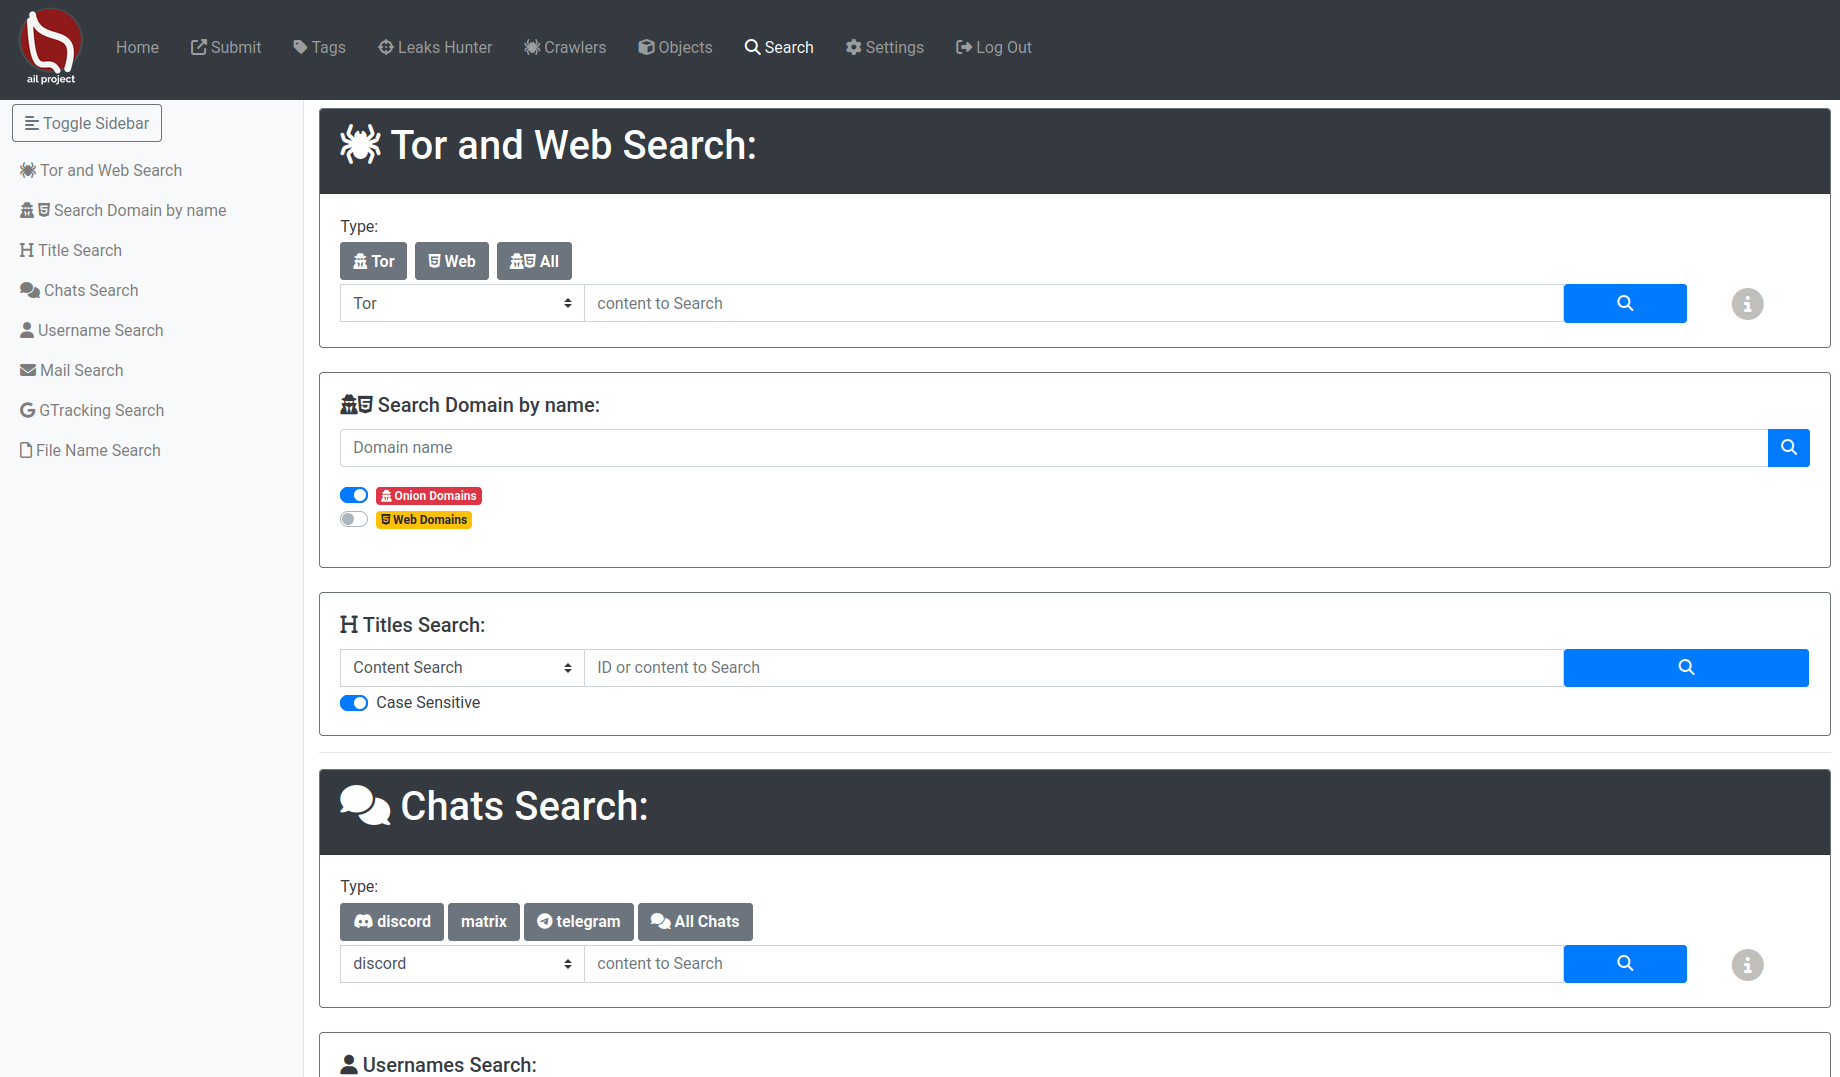
\includegraphics[scale=0.18, angle=0]{screenshot/search.png}
    \end{figure}
\end{frame}

\begin{frame}
    \frametitle{YARA Tracker}
        \begin{figure}
            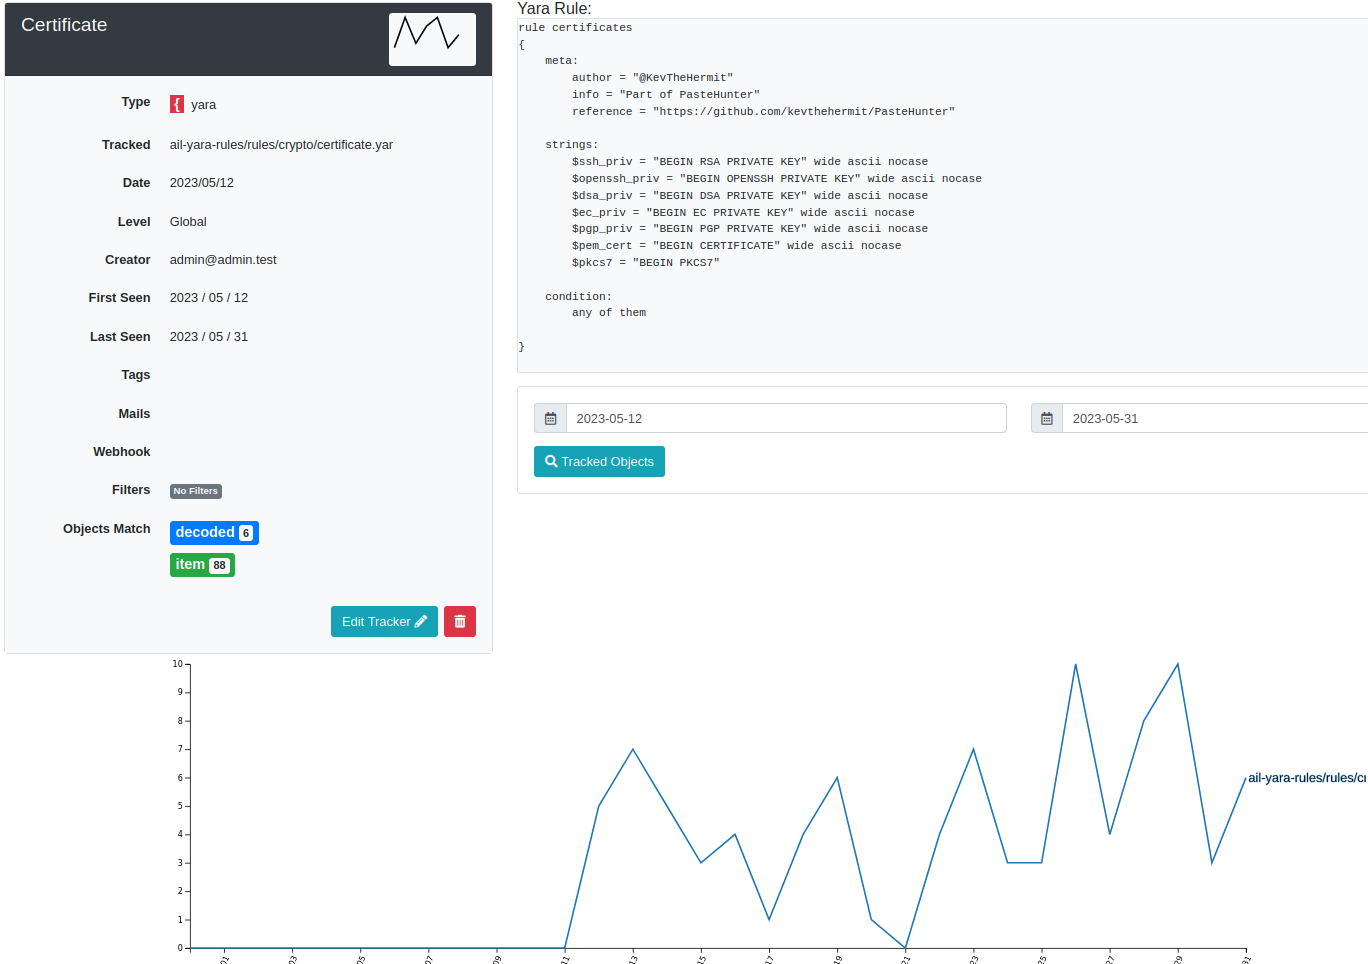
\includegraphics[scale=0.22]{screenshot/tracker_yara.png}
        \end{figure}
\end{frame}

\begin{frame}
    \frametitle{Retro Hunt}
        \begin{figure}
            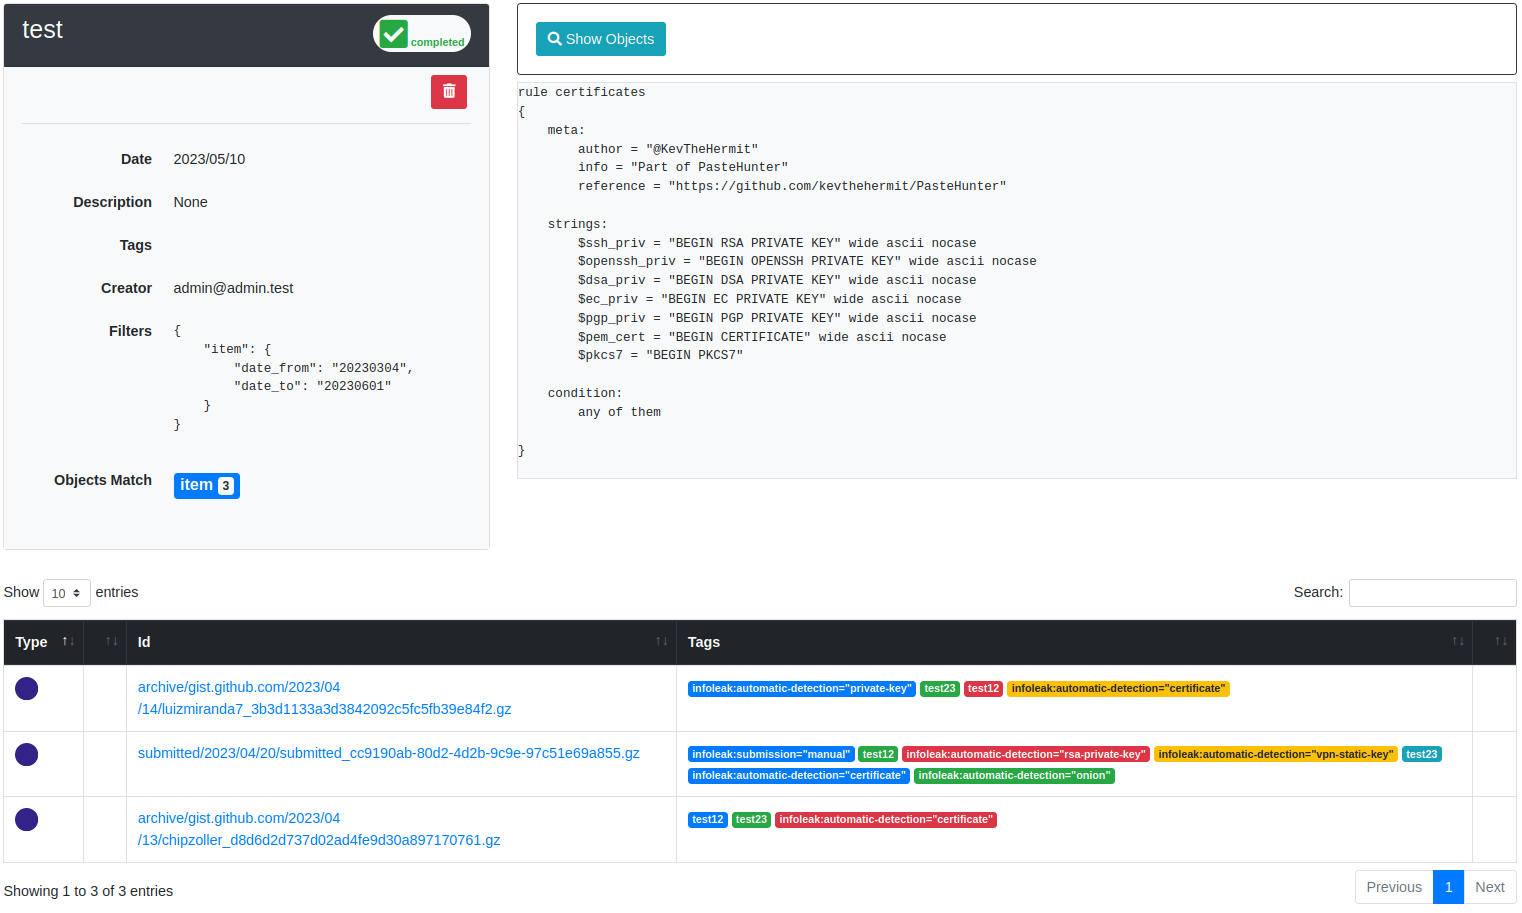
\includegraphics[scale=0.22]{screenshot/retro_hunt.png}
        \end{figure}
\end{frame}


\begin{frame}
    \frametitle{Correlations and relationship}
    \begin{figure}
        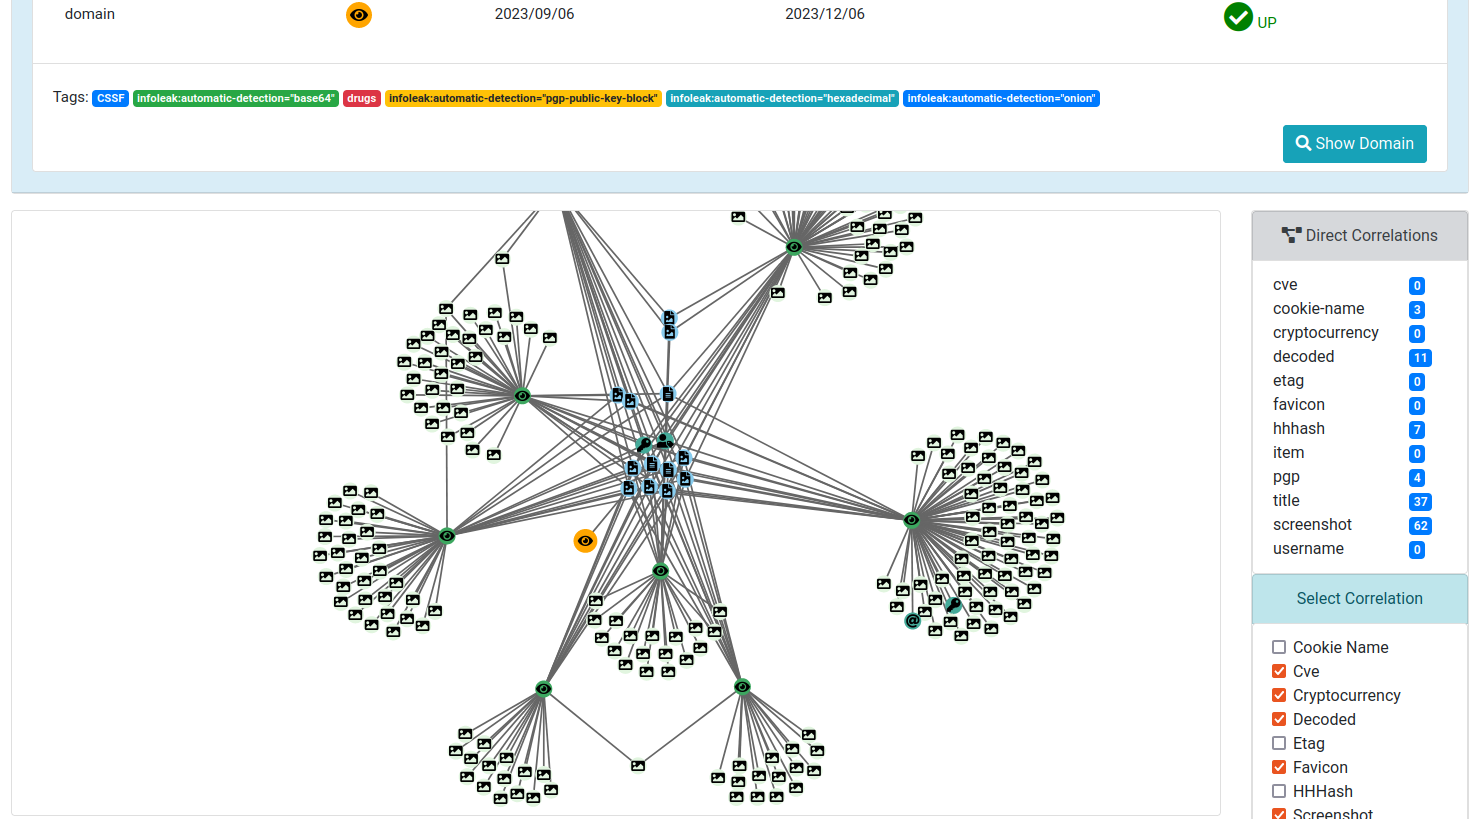
\includegraphics[scale=0.23, angle=0]{screenshot/ail-correlation.png}
    \end{figure}
\end{frame}

\begin{frame}
    \frametitle{User Correlation - Common Chats}
    \begin{center}
        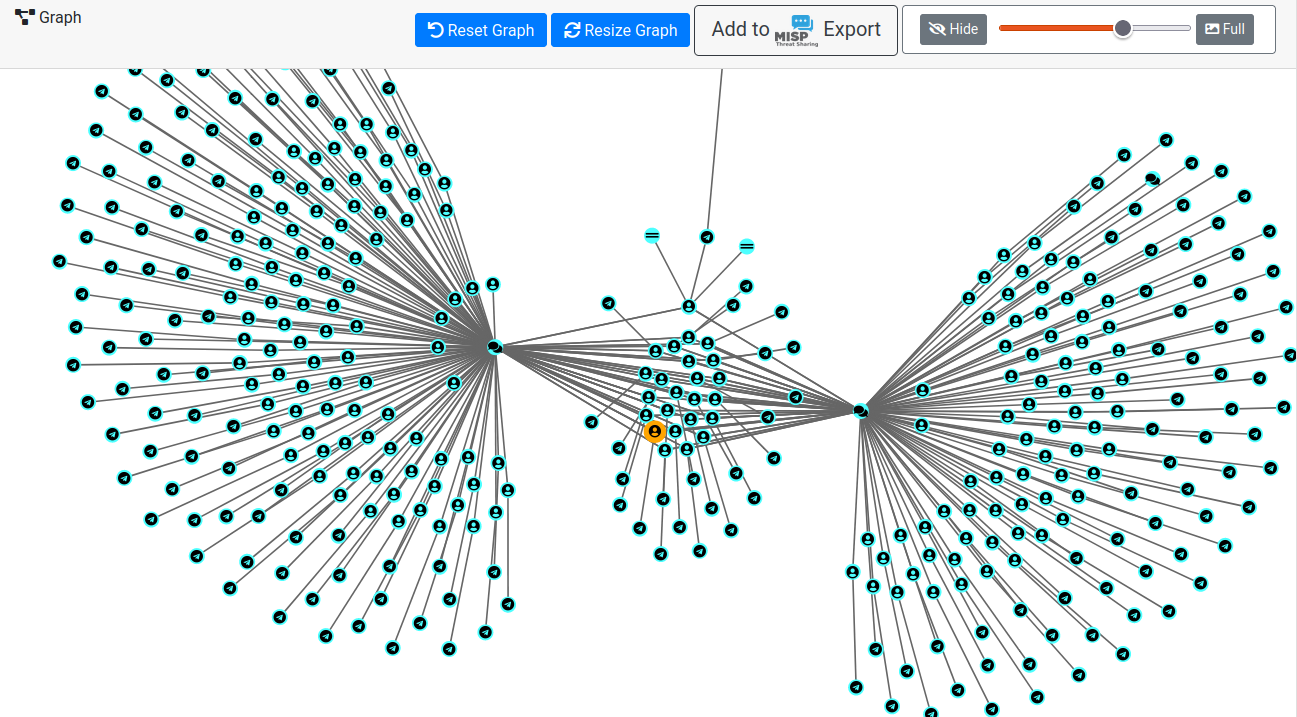
\includegraphics[scale=0.26]{screenshot/chat_users_correlation.png}
    \end{center}
\end{frame}

\begin{frame}
    \frametitle{What are the Relationships Between Chats Group?}
    \begin{center}
        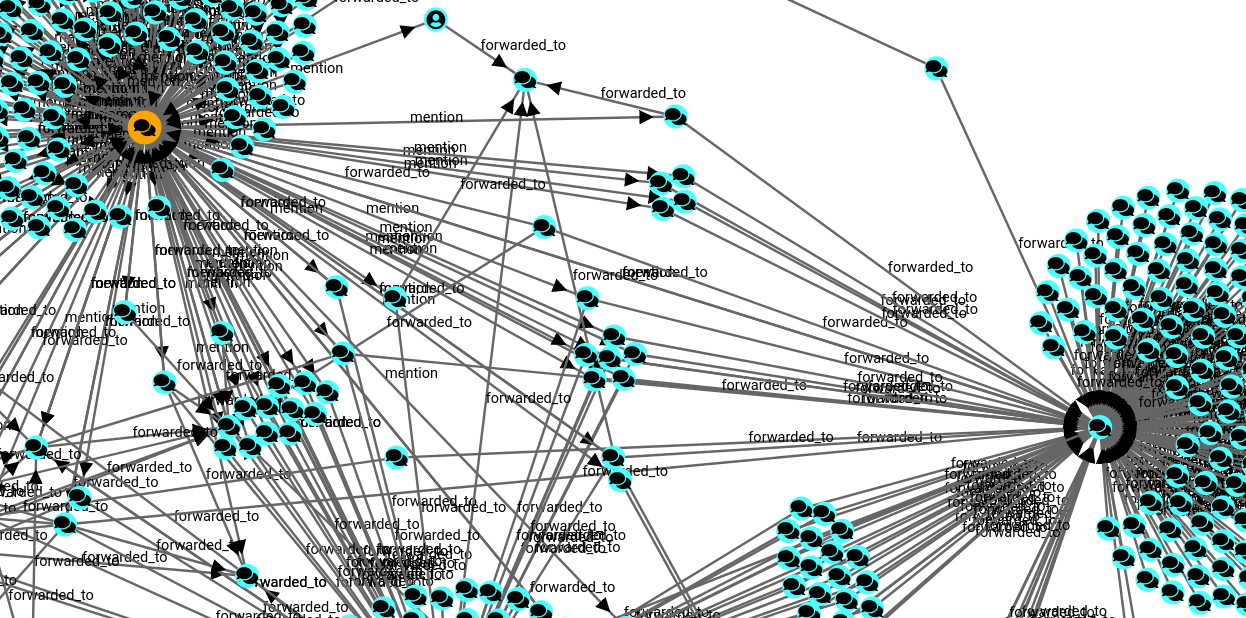
\includegraphics[scale=0.27]{screenshot/noname-relationships.png}
    \end{center}
\end{frame}

\begin{frame}
    \frametitle{Investigations}
    \begin{figure}
        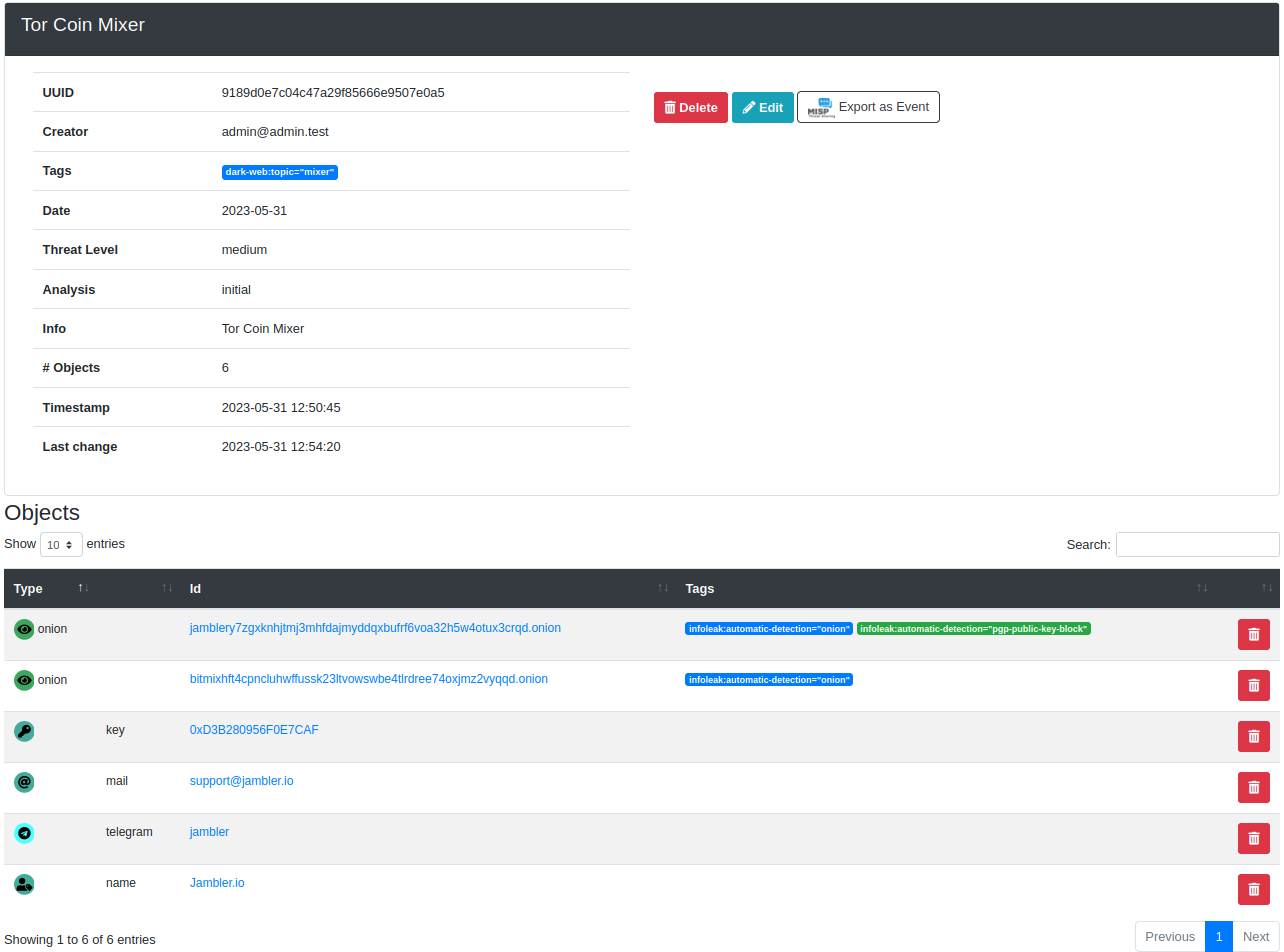
\includegraphics[scale=0.22, angle=0]{screenshot/investigation_mixer.png}
    \end{figure}
\end{frame}

\begin{frame}
    \frametitle{AIL Framework: Extensible Capabilities}
    \begin{itemize}
        \item Extending AIL to add a new \textbf{analysis module} can be done in 50 lines of Python.
        \item The framework \textbf{supports multi-processors/cores by default}. Any analysis module can be started multiple times to support faster processing during peak times or bulk import.
        \item \textbf{Multiple} concurrent \textbf{data inputs}.
        \item Tor Crawler (handles cookies and authentication).
        \item Feeders: Discord, Telegram, ...
    \end{itemize}
\end{frame}


\begin{frame}
    \frametitle{Ongoing Developments}
    \begin{itemize}
        \item \textbf{Improved Mail Search – Next Release}
        \item \textbf{Lacus crawler improvements:} proxy selection, local cache, and cookie state transfer
        \item \textbf{Distributed Image Description Processing} - Automatic load balancing and per-domain classification across multiple Ollama servers
        \item \textbf{Translate search:} support for searching in other languages
        \item \textbf{Advanced video processing and extraction}
        \item \textbf{MISP export with new correlation types}
        \item \textbf{Automatic geolocation}
    \end{itemize}
\end{frame}

% LINKS
\begin{frame}
\frametitle{Links}
    \begin{itemize}
        \item AIL project website \url{https://ail-project.org}
        \item AIL project open source framework \url{https://github.com/ail-project}
        \item Training materials \url{https://github.com/ail-project/ail-training}
        \item Online chat \url{https://gitter.im/ail-project/community}
    \end{itemize}
    \begin{figure}
        
\includegraphics[scale=0.1, angle=0]{images/ail-project.png}
    \end{figure}
\end{frame}

%\begin{frame}
%    \frametitle{\textbf{MISP - LEA}}
%    \begin{itemize}
%        \item Law Enforcement Agency Information Sharing Community
%        \item AIL-LEA instance hosted by CIRCL
%        \item Request access by sending an email to \textbf{info@misp-lea.org} or \textbf{info@circl.lu}
%        \item Request free training at \textbf{info@misp-lea.org} or \textbf{info@circl.lu}
%    \end{itemize}
%    \begin{center}
%        
\includegraphics[scale=0.3]{images/misp-lea.png}
%    \end{center}
%\end{frame}

\begin{frame}
	\frametitle{Thank you for your attention}
	\begin{itemize}
		\item AIL project\footnote{All techniques and indicators mentioned in these slides are implemented in the AIL project, using an instance backed by a three-year dataset collected from Tor hidden services and various social networks.}
: \url{https://github.com/ail-project/ail-framework}
		\item For questions, contact: \href{mailto:info@circl.lu}{info@circl.lu}
	\end{itemize}
\end{frame}
\end{document}
